% Provenance (never printed): see sources/outline_sources.md (Year 1: insolation with
% latitude and season, the radiative surplus and deficit, meridional heat transport by
% the atmosphere and the ocean, latent heat). Exercise and problem values in the Book 3
% scratch calculator calc/ch27.py; figures from figdata/bachelor-1/insolation.py (Kepler
% orbit of _solar.py) and energy_balance.py (NCEP-NCAR Reanalysis 1, long-term means
% 1991-2020, datasets bachelor-1-ncep-*).
% Physics owns the inverse-square law, the black body and the Stefan-Boltzmann law, the
% seasons and latent heat (recalled). Book 2 (g10) gave the quarter of the solar constant,
% the global budget diagram and its closure, latent and sensible heat in words, the
% annual-mean insolation curve and the poleward transport in words: re-founded here with
% derivations and data. Ch. 1 gave the instantaneous insolation, the declination and the
% rising and setting of the Sun.
\chapter{Le rayonnement et le transport de chaleur}\label{ch:b1:radiation-heat-transport}

À un million de milles, la face éclairée de la Terre est un disque de mer bleue,
de terre brune et de nuages blancs. La lumière du Soleil tombe le plus directement au milieu du
disque, près des tropiques, et rase ses bords~; les tropiques absorbent bien plus
d'énergie que les régions polaires. Pourtant les tropiques ne se réchauffent pas d'année en
année, ni les pôles ne se refroidissent. Les vents et les courants océaniques portent l'excédent vers
les pôles, plusieurs pétawatts. Ce chapitre mesure les trois termes de ce bilan~:
la lumière solaire que reçoit chaque \omterm{def:b1:spherical-astronomy:geographic}{latitude}, la part qu'elle garde et l'infrarouge qu'elle renvoie
vers l'espace, et le transport qui compense la différence. Une grande part du
transport voyage sous une forme invisible, la vapeur d'eau, dont la chaleur latente est
libérée partout où elle se condense en pluie.
% ledger: commons:epic-earth, trenberth:transport

\begin{omfigure}
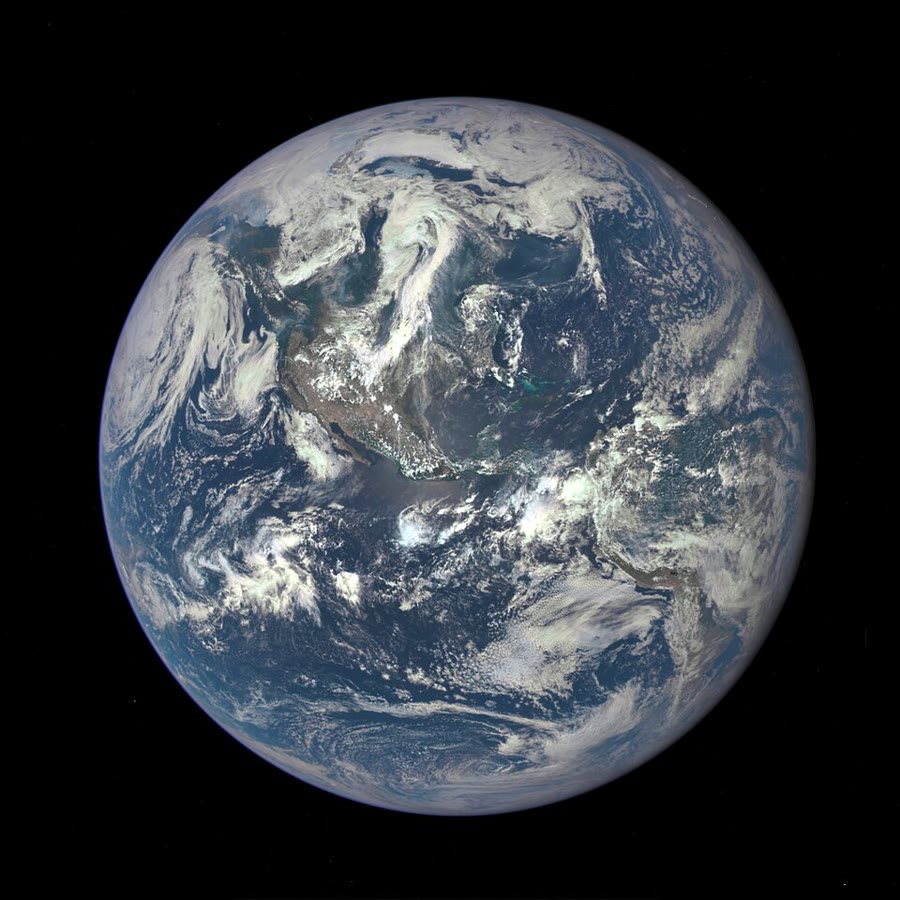
\includegraphics[width=0.55\linewidth]{images/book3/b1-epic-earth.jpg}

{\small Tout le côté éclairé de la Terre, photographié le 6~juillet 2015 par une
caméra du Deep Space Climate Observatory, à un million de milles~; l'Amérique du Nord et
centrale sont au milieu, avec les mers peu profondes turquoise des
Caraïbes. Deux semaines après le solstice de juin l'Arctique, en haut, est éclairé
jour et nuit. Les nuages brillants réfléchissent une grande part de la lumière qui les atteint~; la teinte bleutée est de la
lumière solaire diffusée par les molécules de l'air. (NASA Goddard Space Flight Center,
domaine public, via Wikimedia Commons.)}
\label{fig:b1:radiation-heat-transport:epic}
\end{omfigure}
% ledger: commons:epic-earth (polar day: figdata/bachelor-1/insolation.py)

\begin{recall}
Le \cref{ch:b1:spherical-astronomy} a défini l'\omterm{def:b1:spherical-astronomy:insolation}{insolation}, la puissance de la lumière du Soleil
reçue par mètre carré d'une surface horizontale au sommet de l'atmosphère,
$I = S_0(a/r)^2\sin h_\odot$ tant que le Soleil est levé, avec $S_0 = \qty{1361}{W.m^{-2}}$
à la distance moyenne $a$~; il a donné la hauteur du Soleil d'après son \omterm{def:b1:spherical-astronomy:equatorial}{angle horaire} $H$, sa
\omterm{def:b1:spherical-astronomy:equatorial}{déclinaison} $\delta$ et la \omterm{def:b1:spherical-astronomy:geographic}{latitude} $\varphi$,
$\sin h_\odot = \sin\varphi\sin\delta + \cos\varphi\cos\delta\cos H$~; et l'\omterm{def:b1:spherical-astronomy:equatorial}{angle
horaire} $H_0$ du coucher, $\cos H_0 = -\tan\varphi\tan\delta$
(\cref{prop:b1:spherical-astronomy:rising}). Le \cref{ch:b1:comparative-planetology}
a défini l'\omterm{def:b1:comparative-planetology:albedo}{albédo de Bond} d'une planète et sa \omterm{def:b1:comparative-planetology:equilibrium-temperature}{température d'équilibre}. Les volumes de
physique donnent la loi en inverse du carré pour la lumière, le rayonnement d'un corps noir,
$\sigma T^4$ par mètre carré avec $\sigma = \qty{5.670e-8}{W.m^{-2}.K^{-4}}$
(Stefan--Boltzmann), et la chaleur latente d'un changement d'état. Le livre~2 a montré que
la Terre intercepte en moyenne le quart de la constante solaire, a dessiné le bilan
énergétique global de la Terre et vérifié qu'il s'équilibre, et a décrit le
transport de chaleur vers les pôles en mots.
% ledger: earth:TSI, const:sigma, ipcc:budget-toa
\end{recall}

\section{L'insolation selon la latitude et la saison}\label{sec:b1:radiation-heat-transport:insolation}

L'\omterm{def:b1:spherical-astronomy:insolation}{insolation} instantanée change de minute en minute à mesure que le Soleil traverse le
ciel. Pour le climat, ce qui compte est sa somme sur un jour.

\begin{definition}[Insolation journalière moyenne]\label{def:b1:radiation-heat-transport:daily-insolation}
L'\emph{insolation journalière moyenne}\index{insolation journaliere moyenne@insolation journalière moyenne} $\bar Q$ à une \omterm{def:b1:spherical-astronomy:geographic}{latitude}
un jour donné est l'\omterm{def:b1:spherical-astronomy:insolation}{insolation} instantanée moyennée sur les 24 heures de ce
jour, nuits comprises, la \omterm{def:b1:spherical-astronomy:equatorial}{déclinaison} du Soleil et sa distance étant tenues à
leurs valeurs du jour. C'est une puissance par mètre carré de surface horizontale au
sommet de l'atmosphère, en \unit{W.m^{-2}}.
\end{definition}

Tenir $\delta$ et $r$ fixes pendant un jour est sans danger~: la \omterm{def:b1:spherical-astronomy:equatorial}{déclinaison} change
d'au plus \ang{0.4} par jour, et la distance de moins de \qty{0.03}{\percent}.
% ledger: earth:obliquity, earth:ecc (computed in figdata/bachelor-1/insolation.py)

\begin{theorem}[Insolation journalière moyenne]\label{thm:b1:radiation-heat-transport:daily}
À la \omterm{def:b1:spherical-astronomy:geographic}{latitude} $\varphi$, un jour où la \omterm{def:b1:spherical-astronomy:equatorial}{déclinaison} du Soleil est $\delta$ et sa
distance $r$,
\[
  \bar Q = \frac{S_0}{\pi}\left(\frac{a}{r}\right)^{2}
  \bigl(h_0\sin\varphi\sin\delta + \cos\varphi\cos\delta\sin h_0\bigr),
\]
où $h_0 \in [0, \pi]$ est l'\omterm{def:b1:spherical-astronomy:equatorial}{angle horaire} du coucher en radians~: $\cos h_0 =
-\tan\varphi\tan\delta$ quand $|\tan\varphi\tan\delta| \le 1$~; $h_0 = \pi$ dans le
jour polaire ($\tan\varphi\tan\delta > 1$)~; $h_0 = 0$, et $\bar Q = 0$, dans la nuit
polaire ($\tan\varphi\tan\delta < -1$).
\end{theorem}

\begin{proof}
L'\omterm{def:b1:spherical-astronomy:equatorial}{angle horaire} $H$ avance uniformément de $2\pi$ en un jour, donc la moyenne sur
le jour est la moyenne sur $H \in [-\pi, \pi]$. Le Soleil est levé pour $-h_0 < H < h_0$,
où $\sin h_\odot > 0$, et l'\omterm{def:b1:spherical-astronomy:insolation}{insolation} est nulle ailleurs. D'où
\[
  \bar Q = \frac{1}{2\pi}\int_{-h_0}^{h_0} S_0\left(\frac{a}{r}\right)^{2}
  \bigl(\sin\varphi\sin\delta + \cos\varphi\cos\delta\cos H\bigr)\,\mathrm dH ,
\]
qui vaut $(S_0/2\pi)(a/r)^2\bigl(2h_0\sin\varphi\sin\delta +
2\cos\varphi\cos\delta\sin h_0\bigr)$.
Les bornes viennent de la \cref{prop:b1:spherical-astronomy:rising}~: la hauteur est
nulle quand $\cos H = -\tan\varphi\tan\delta$. Si ce nombre dépasse 1 en valeur
absolue, le Soleil ne franchit jamais l'horizon~: quand $\tan\varphi\tan\delta > 1$,
l'intégrande est positive pour tout $H$ et l'intégrale porte sur le jour entier,
$h_0 = \pi$~; quand $\tan\varphi\tan\delta < -1$, elle est négative pour tout $H$ et
le Soleil ne se lève jamais.
\end{proof}

Deux cas particuliers valent d'être sus par cœur. À l'équateur, $\varphi = 0$ et
$h_0 = \pi/2$ quelle que soit la saison~:
\[
  \bar Q_\text{équateur} = \frac{S_0}{\pi}\left(\frac{a}{r}\right)^{2}\cos\delta ,
\]
maximale aux équinoxes, $S_0/\pi = \qty{433.2}{W.m^{-2}}$ à la distance moyenne.
À un pôle en été, $h_0 = \pi$ et $\varphi = \pi/2$~: $\bar Q_\text{pôle} =
S_0(a/r)^2\sin\delta$, le Soleil tournant dans le ciel à une hauteur constante égale à
la \omterm{def:b1:spherical-astronomy:equatorial}{déclinaison}.
% ledger: earth:TSI

\begin{proposition}[L'été polaire]\label{prop:b1:radiation-heat-transport:polar-summer}
Un jour de \omterm{def:b1:spherical-astronomy:equatorial}{déclinaison} $\delta > 0$, l'\omterm{def:b1:radiation-heat-transport:daily-insolation}{insolation journalière moyenne} au pôle Nord
dépasse celle à l'équateur si et seulement si $\pi\tan\delta > 1$, c'est-à-dire $\delta >
\ang{17.66}$. Au solstice de juin, $\delta = \ang{23.44}$, le rapport est $\pi\tan
\delta = 1.362$.
\end{proposition}

\begin{proof}
Les deux cas particuliers ci-dessus partagent le facteur $(S_0/\pi)(a/r)^2$~; leur rapport est
$\pi\sin\delta/\cos\delta = \pi\tan\delta$, qui dépasse 1 quand $\tan\delta >
1/\pi$, $\delta > \arctan(1/\pi) = \ang{17.66}$. Avec l'obliquité,
$\pi\tan\ang{23.44} = 1.362$.
\end{proof}
% ledger: earth:obliquity

Avec l'orbite de la Terre, le solstice de juin tombe près de l'aphélie, $(a/r)^2 = 0.968$~:
le pôle Nord reçoit alors \qty{524}{W.m^{-2}} en moyenne journalière, l'équateur
\qty{385}{W.m^{-2}}. Six mois plus tard le pôle Sud, près du périhélie, reçoit
\qty{559}{W.m^{-2}}, \qty{6.7}{\percent} de plus que le pôle Nord dans son
été~: le rapport est exactement celui des deux valeurs de $(a/r)^2$. La figure ci-dessous
montre $\bar Q$ sur toute une année. Les maxima sont aux pôles aux solstices~;
les coins sombres sont les nuits polaires, limitées par la \omterm{def:b1:spherical-astronomy:geographic}{latitude} $\ang{90} -
|\delta|$~; le point subsolaire, où le Soleil passe au \omterm{def:b1:spherical-astronomy:celestial-sphere}{zénith} à midi, se déplace
entre les tropiques avec la \omterm{def:b1:spherical-astronomy:equatorial}{déclinaison}.
% ledger: earth:TSI, earth:ecc, earth:obliquity, nasa:earth-perihelion-longitude, usno:seasons-2026 (computed in figdata/bachelor-1/insolation.py)

\begin{omfigure}
\begin{tikzpicture}
\begin{axis}[omrecord, width=0.8\linewidth, height=6.4cm, view={0}{90},
  xmin=0, xmax=365, ymin=-90, ymax=90, xlabel={jour de l'année (depuis le {1\textsuperscript{er}} janvier)},
  ylabel={latitude (\unit{\degree})}, xtick={0,60,...,360}, ytick={-90,-60,...,90},
  colormap/viridis, colorbar, point meta min=0, point meta max=560,
  colorbar style={ylabel={$\bar Q$ (\unit{W.m^{-2}})}, ytick={0,100,...,500}, width=0.3cm},
  axis on top, grid=none]
% figdata/bachelor-1/insolation.py; ledger: earth:TSI, earth:ecc, earth:obliquity, nasa:earth-perihelion-longitude, usno:tropical-year, usno:seasons-2026
\addplot3[surf, shader=interp, mesh/ordering=y varies, mesh/rows=73]
  table[x=day, y=lat, z=Q] {figdata/out/bachelor-1-insolation-grid.dat};
\addplot3[white, dashed, line width=0.8pt] table[x=day, y=decl, z expr=600] {figdata/out/bachelor-1-insolation-sun.dat};
\addplot3[white, line width=0.6pt, unbounded coords=jump] table[x=day, y=night_n, z expr=600] {figdata/out/bachelor-1-insolation-sun.dat};
\addplot3[white, line width=0.6pt, unbounded coords=jump] table[x=day, y=night_s, z expr=600] {figdata/out/bachelor-1-insolation-sun.dat};
\node[font=\scriptsize, text=white] at (axis cs:28,81,700) {nuit polaire};
\node[font=\scriptsize, text=white] at (axis cs:172,-81,700) {nuit polaire};
\node[font=\scriptsize, text=white, anchor=south] at (axis cs:172,26,700) {latitude subsolaire};
\end{axis}
\end{tikzpicture}

{\small \omterm{def:b1:radiation-heat-transport:daily-insolation}{Insolation journalière moyenne} au sommet de l'atmosphère en fonction du jour de
l'année et de la \omterm{def:b1:spherical-astronomy:geographic}{latitude}, d'après le \cref{thm:b1:radiation-heat-transport:daily} avec
$S_0 = \qty{1361}{W.m^{-2}}$ et l'orbite de la Terre. Tirets~: la \omterm{def:b1:spherical-astronomy:geographic}{latitude} subsolaire,
égale à la \omterm{def:b1:spherical-astronomy:equatorial}{déclinaison}~; trait plein~: les bords des nuits polaires. Les pôles d'été
reçoivent plus que tout autre endroit de la Terre~; l'été austral, près du
périhélie, est le plus lumineux des deux.}
\label{fig:b1:radiation-heat-transport:matrix}
\end{omfigure}
% ledger: earth:TSI, earth:ecc, earth:obliquity, nasa:earth-perihelion-longitude, usno:seasons-2026

La moyenne de $\bar Q$ sur l'année donne l'\omterm{def:b1:spherical-astronomy:insolation}{insolation} annuelle moyenne de chaque \omterm{def:b1:spherical-astronomy:geographic}{latitude}
(figure ci-dessous)~: \qty{415.6}{W.m^{-2}} à l'équateur, \qty{328.3}{W.m^{-2}} à
\ang{40}, \qty{172.4}{W.m^{-2}} à l'un ou l'autre pôle. L'été polaire est intense mais
l'hiver polaire est sombre, et sur une année l'équateur reçoit \num{2.41} fois autant
qu'un pôle. La courbe est la même dans les deux hémisphères, bien que l'été austral
soit le plus lumineux~; l'\cref{exo:b1:radiation-heat-transport:10} montre pourquoi.
% ledger: earth:TSI, earth:ecc, earth:obliquity (computed in figdata/bachelor-1/insolation.py)

\begin{omfigure}
\begin{tikzpicture}
\begin{axis}[omrecord, width=0.8\linewidth, height=5.6cm, xmin=-90, xmax=90, ymin=0, ymax=600,
  xlabel={latitude (\unit{\degree})}, ylabel={$\bar Q$ (\unit{W.m^{-2}})},
  xtick={-90,-60,...,90}, ytick={0,100,...,600}]
% figdata/bachelor-1/insolation.py; ledger: earth:TSI, earth:ecc, earth:obliquity, nasa:earth-perihelion-longitude
\addplot[omThm, line width=0.8pt] table[x=lat, y=Q_jun] {figdata/out/bachelor-1-insolation-annual.dat};
\addplot[omDef, line width=0.8pt] table[x=lat, y=Q_dec] {figdata/out/bachelor-1-insolation-annual.dat};
\addplot[black, line width=1.1pt] table[x=lat, y=Q_ann] {figdata/out/bachelor-1-insolation-annual.dat};
\addplot[black!60, dashed, domain=-90:90] {340.30};
\node[font=\scriptsize, text=omThm, anchor=west] at (axis cs:50,540) {solstice de juin};
\node[font=\scriptsize, text=omDef, anchor=north west] at (axis cs:-88,478) {solstice de décembre};
\node[font=\scriptsize, anchor=north] at (axis cs:-72,160) {moyenne annuelle};
\node[font=\scriptsize, text=black!60, anchor=south west] at (axis cs:-88,342) {moyenne globale};
\end{axis}
\end{tikzpicture}

{\small \omterm{def:b1:radiation-heat-transport:daily-insolation}{Insolation journalière moyenne} en fonction de la \omterm{def:b1:spherical-astronomy:geographic}{latitude} aux deux solstices, et sa
moyenne annuelle (noir). La moyenne annuelle dépasse la moyenne globale, \qty{340.3}{W.m^{-2}}
(tirets), entre \ang{37}~S et \ang{37}~N, sur \qty{60}{\percent} de la surface
de la Terre.}
\label{fig:b1:radiation-heat-transport:annual}
\end{omfigure}
% ledger: earth:TSI, earth:ecc, earth:obliquity (computed in figdata/bachelor-1/insolation.py)

\begin{proposition}[La moyenne globale]\label{prop:b1:radiation-heat-transport:global}
À chaque instant, l'\omterm{def:b1:spherical-astronomy:insolation}{insolation} moyennée sur toute la sphère est $\tfrac14
S_0(a/r)^2$. Moyennée aussi sur l'année, elle est $S_0/(4\sqrt{1 - e^2})$, où
$e$ est l'excentricité de l'orbite~: \qty{340.30}{W.m^{-2}} pour la Terre, à
\qty{0.02}{\percent} de $S_0/4 = \qty{340.25}{W.m^{-2}}$.
\end{proposition}

\begin{proof}
La Terre, de rayon $R$, intercepte la lumière du Soleil qui traverse un disque d'aire $\pi
R^2$, une puissance $S_0(a/r)^2\pi R^2$, qui tombe sur l'hémisphère éclairé~; répartie sur
toute la surface $4\pi R^2$, elle donne le premier résultat. La moyenne temporelle de
$(a/r)^2$ sur l'orbite est $1/\sqrt{1-e^2}$
(\cref{exo:b1:radiation-heat-transport:11}).
\end{proof}
% ledger: earth:TSI, earth:ecc

\section{Rayonnement absorbé et émis}\label{sec:b1:radiation-heat-transport:toa}

De la lumière du Soleil qu'une \omterm{def:b1:spherical-astronomy:geographic}{latitude} reçoit, elle en réfléchit une fraction directement, par les
nuages, la neige, la glace, le désert et, à un moindre degré, la mer~; elle absorbe le reste, dans
l'air et à la surface. Elle perd aussi de l'énergie en émettant du rayonnement infrarouge
vers l'espace, jour et nuit.

\begin{definition}[Rayonnement infrarouge sortant]\label{def:b1:radiation-heat-transport:olr}
Le \emph{rayonnement infrarouge sortant}\index{rayonnement infrarouge sortant} (OLR, de l'anglais \textit{outgoing longwave radiation})
est la puissance de rayonnement infrarouge quittant le sommet de l'atmosphère vers l'espace,
par mètre carré. La \emph{température d'émission}\index{temperature d'emission@température d'émission}
$T_e$ est la température d'un corps noir qui émettrait la même puissance~:
$\sigma T_e^4 = \text{OLR}$.
\end{definition}

L'OLR vient en partie de la surface, à travers l'air là où il est transparent
à l'infrarouge, et en partie de l'air et des sommets de nuages plus haut. La \omterm{def:b1:radiation-heat-transport:olr}{température d'émission}
est une propriété du
rayonnement, non la température d'un niveau particulier~: elle est plus basse que celle
du sol en dessous, parce que les couches émettrices sont plus froides.
% ledger: ipcc:budget-surface, ipcc:budget-toa

\begin{definition}[Rayonnement net~; excédent et déficit radiatifs]\label{def:b1:radiation-heat-transport:net-radiation}
Le \emph{rayonnement net}\index{rayonnement net} au sommet de l'atmosphère est
\[
  R = \underbrace{(1 - \alpha)\,\bar Q}_{\text{solaire absorbé}} - \text{OLR},
\]
où $\alpha$ est l'albédo local, la fraction de la lumière du Soleil incidente réfléchie
vers l'espace~; les trois grandeurs sont des moyennes annuelles à une \omterm{def:b1:spherical-astronomy:geographic}{latitude}. Une \omterm{def:b1:spherical-astronomy:geographic}{latitude} où
$R > 0$ a un \emph{excédent radiatif}\index{excedent radiatif@excédent radiatif}~; une où $R < 0$
a un \emph{déficit radiatif}\index{deficit radiatif@déficit radiatif}.
\end{definition}

Sur toute la Terre le \omterm{def:b1:radiation-heat-transport:net-radiation}{rayonnement net} doit avoir une moyenne presque nulle, puisque la planète
ne se réchauffe ni ne se refroidit de plus de quelques dixièmes de watt par mètre carré~: la
dernière évaluation place le déséquilibre à \qty{0.7}{W.m^{-2}}, sur un flux incident de
\qty{340}{W.m^{-2}} dont \qty{100}{W.m^{-2}} sont réfléchis (un albédo global de
\num{0.294}) et \qty{239}{W.m^{-2}} repartent sous forme d'infrarouge.
% ledger: ipcc:budget-toa, earth:albedo

Les profils zonaux de ce chapitre viennent d'une réanalyse, c'est-à-dire d'un système de
prévision météorologique exécuté sur les décennies passées, qui assimile les observations de
chaque jour et fournit un état complet et cohérent de l'atmosphère. La
réanalyse utilisée ici, à partir de 1948, donne des moyennes mensuelles sur une grille de 94 \omterm{def:b1:spherical-astronomy:geographic}{latitudes}
et 192 \omterm{def:b1:spherical-astronomy:geographic}{longitudes}~; ce chapitre utilise ses moyennes sur 1991--2020. Ses flux de rayonnement
sont des sorties de modèle, des prévisions contraintes par les observations. La figure
ci-dessous montre leurs moyennes zonales en fonction de $\sin\varphi$, de sorte que des largeurs égales sur
l'axe sont des aires égales sur la sphère.
% ledger: psl:ncep-r1, kalnay96:reanalysis, data:b3-ncep

\begin{omfigure}
\begin{tikzpicture}
\begin{axis}[omrecord, width=0.8\linewidth, height=6cm, xmin=-1, xmax=1, ymin=0, ymax=320,
  xlabel={latitude (\unit{\degree}, axe en $\sin\varphi$)}, ylabel={flux (\unit{W.m^{-2}})},
  xtick={-0.866,-0.5,0,0.5,0.866}, xticklabels={60 S,30 S,0,30 N,60 N},
  ytick={0,50,...,300}]
% figdata/bachelor-1/energy_balance.py; ledger: data:b3-ncep, psl:ncep-r1
\addplot[name path=asr, omProp, line width=1pt] table[x expr={sin(\thisrow{lat})}, y=asr] {figdata/out/bachelor-1-energy_balance-toa.dat};
\addplot[name path=olr, omThm, line width=1pt] table[x expr={sin(\thisrow{lat})}, y=olr] {figdata/out/bachelor-1-energy_balance-toa.dat};
\addplot[omProp!25] fill between[of=asr and olr, split, every segment no 1/.style={omDef!18}, every segment no 2/.style={omProp!30}, every segment no 3/.style={omDef!18}];
\node[font=\scriptsize, text=omProp!80!black] at (axis cs:-0.55,300) {solaire absorbé};
\node[font=\scriptsize, text=omThm] at (axis cs:-0.2,226) {OLR};
\node[font=\scriptsize] at (axis cs:0,262) {excédent};
\node[font=\scriptsize] at (axis cs:0.86,178) {déficit};
\node[font=\scriptsize] at (axis cs:-0.86,178) {déficit};
\end{axis}
\end{tikzpicture}

{\small Rayonnement solaire absorbé (orange) et \omterm{def:b1:radiation-heat-transport:olr}{rayonnement infrarouge sortant}
(rouge) en moyenne zonale et annuelle au sommet de l'atmosphère, d'après la
Réanalyse~1 NCEP-NCAR, moyennes 1991--2020 (données fournies par le NOAA PSL, Boulder, Colorado,
États-Unis, depuis leur site https://psl.noaa.gov). Zones teintées~: l'\omterm{def:b1:radiation-heat-transport:net-radiation}{excédent radiatif} des
basses \omterm{def:b1:spherical-astronomy:geographic}{latitudes} et les déficits des hautes \omterm{def:b1:spherical-astronomy:geographic}{latitudes}.}
\label{fig:b1:radiation-heat-transport:toa}
\end{omfigure}
% ledger: data:b3-ncep, psl:ncep-r1, kalnay96:reanalysis

Les deux courbes ont des formes très différentes. La lumière solaire absorbée chute de
\qty{288}{W.m^{-2}} près de l'équateur à \qty{76}{W.m^{-2}} à \ang{81}~N, d'un
facteur \num{3.8}~: l'\omterm{def:b1:spherical-astronomy:insolation}{insolation} baisse, et l'albédo passe de \num{0.31} à
\num{0.57}, avec le Soleil bas, la neige et la glace de mer. L'OLR ne chute que de
\qty{245}{W.m^{-2}} à \qty{192}{W.m^{-2}}, d'un facteur \num{1.27}~; les
\omterm{def:b1:radiation-heat-transport:olr}{températures d'émission} sont \qty{256}{K} et \qty{241}{K}. L'OLR est même légèrement
plus bas à l'équateur, \qty{245}{W.m^{-2}}, que près de \ang{20}, \qty{269}{W.m^{-2}}~:
les nuages de la ceinture de pluie équatoriale montent haut et leurs sommets froids émettent peu,
tandis que les cieux subtropicaux plus clairs laissent s'échapper davantage d'infrarouge. Partout où la lumière solaire absorbée dépasse l'OLR, la \omterm{def:b1:spherical-astronomy:geographic}{latitude} a un
excédent.
% ledger: data:b3-ncep (values computed in figdata/bachelor-1/energy_balance.py)

\begin{example}[Le bilan global de la réanalyse]\label{ex:b1:radiation-heat-transport:global}
En moyenne sur le globe, la réanalyse reçoit \qty{341.9}{W.m^{-2}}, réfléchit
\qty{117.0}{W.m^{-2}} (un albédo de \num{0.342}), absorbe \qty{224.8}{W.m^{-2}} et
émet \qty{237.7}{W.m^{-2}}~: un \omterm{def:b1:radiation-heat-transport:net-radiation}{rayonnement net} de \qty{-12.9}{W.m^{-2}}. L'OLR est
à \qty{1.3}{W.m^{-2}} de la valeur évaluée de \qty{239}{W.m^{-2}}, mais la réflexion
est supérieure de \qty{17}{W.m^{-2}} aux \qty{100}{W.m^{-2}} évalués. Un déséquilibre réel
de cette taille refroidirait la Terre de \qty{6.6}{PW}~; c'est une erreur du
modèle, non une propriété de la Terre, et le transport ci-dessous est calculé après
retrait de la moyenne globale.
% ledger: data:b3-ncep, ipcc:budget-toa (computed in figdata/bachelor-1/energy_balance.py)
\end{example}

\section{Le transport méridien de chaleur}\label{sec:b1:radiation-heat-transport:transport}

\begin{definition}[Transport méridien de chaleur]\label{def:b1:radiation-heat-transport:mht}
Le \emph{transport méridien de chaleur}\index{transport meridien de chaleur@transport méridien de chaleur} $T(\varphi)$
à travers le parallèle de \omterm{def:b1:spherical-astronomy:geographic}{latitude} $\varphi$ est l'énergie portée vers le nord à travers
ce parallèle par unité de temps, par l'atmosphère et l'océan ensemble, en moyenne annuelle.
Il est compté positif vers le nord et mesuré en pétawatts
(\qty{1}{PW} = \qty{e15}{W}).
\end{definition}

\begin{proposition}[Le transport d'après le rayonnement net]\label{prop:b1:radiation-heat-transport:mht}
Si l'énergie stockée dans chaque bande de \omterm{def:b1:spherical-astronomy:geographic}{latitude} ne change pas d'une année à l'autre, alors
pour une Terre de rayon $a_\oplus$,
\[
  T(\varphi) = 2\pi a_\oplus^2\int_{-\pi/2}^{\varphi} R(\varphi')\cos\varphi'\,
  \mathrm d\varphi' = -2\pi a_\oplus^2\int_{\varphi}^{\pi/2} R(\varphi')\cos
  \varphi'\,\mathrm d\varphi' ,
\]
et $T$ est extrême aux \omterm{def:b1:spherical-astronomy:geographic}{latitudes} où $R$ change de signe.
\end{proposition}

\begin{proof}
Prenons la calotte polaire au sud du parallèle $\varphi$ comme volume de contrôle, du
fond de l'océan au sommet de l'atmosphère (figure ci-dessous). L'énergie y entre ou en
sort de deux façons seulement~: par rayonnement au sommet, une puissance nette
$\int R\,\mathrm dA$, et par le transport à travers son bord, $-T(\varphi)$ (un
transport vers le nord quitte la calotte sud). La bande entre $\varphi'$ et
$\varphi' + \mathrm d\varphi'$ a pour aire $\mathrm dA = 2\pi a_\oplus\cos\varphi'
\cdot a_\oplus\,\mathrm d\varphi'$. Sans variation de stockage, la somme est nulle~:
$\int_{-\pi/2}^{\varphi} R\,2\pi a_\oplus^2\cos\varphi'\,\mathrm d\varphi' -
T(\varphi) = 0$. Appliqué à la Terre entière ($\varphi = \pi/2$, pas de bord), le même
bilan donne $\int R\,\mathrm dA = 0$ sur la sphère, d'où la seconde forme.
En dérivant, $T'(\varphi) = 2\pi a_\oplus^2 R(\varphi)\cos\varphi$, qui
s'annule là où $R$ change de signe.
\end{proof}
% ledger: earth:Rmean

\begin{omfigure}
\begin{tikzpicture}[>={Stealth[length=2mm]}, font=\scriptsize]
  \def\R{2.0}
  \def\ph{40}
  \fill[omDef!12] ({-\R*cos(\ph)},{\R*sin(\ph)}) arc[start angle=180-\ph, end angle=\ph, radius=\R]
     -- ({\R*cos(\ph)},{\R*sin(\ph)}) arc[start angle=0, end angle=-180, x radius={\R*cos(\ph)}, y radius={0.25*\R*cos(\ph)}] -- cycle;
  \draw[thick] (0,0) circle (\R);
  \draw[black!40] (-\R,0) arc[start angle=180, end angle=360, x radius=\R, y radius={0.25*\R}];
  \draw[black!40, dashed] (\R,0) arc[start angle=0, end angle=180, x radius=\R, y radius={0.25*\R}];
  \draw[omDef, thick] ({-\R*cos(\ph)},{\R*sin(\ph)}) arc[start angle=180, end angle=360, x radius={\R*cos(\ph)}, y radius={0.25*\R*cos(\ph)}];
  \draw[omDef, thick, dashed] ({\R*cos(\ph)},{\R*sin(\ph)}) arc[start angle=0, end angle=180, x radius={\R*cos(\ph)}, y radius={0.25*\R*cos(\ph)}];
  \node[anchor=west, black!60] at (\R+0.05,0) {équateur};
  \node[anchor=west, omDef] at ({\R*cos(\ph)+0.1},{\R*sin(\ph)}) {parallèle $\varphi$};
  \foreach \x in {-0.55,0.55} \draw[->, very thick, omProp] (\x,{\R*sin(\ph)-0.75}) -- (\x,{\R*sin(\ph)-0.1});
  \node[omProp!80!black, anchor=east] at ({-\R-0.1},{\R*sin(\ph)-0.4}) {$T(\varphi)$ traverse le bord};
  \foreach \a in {65,90,115} {
    \draw[->, omThm, decorate, decoration={snake, amplitude=0.6mm, segment length=2mm, post length=1.5mm}]
      ({(\R+0.05)*cos(\a)},{(\R+0.05)*sin(\a)}) -- ({(\R+0.75)*cos(\a)},{(\R+0.75)*sin(\a)});
  }
  \node[omThm, anchor=south] at (0,\R+0.8) {rayonnement net $R < 0$ sur la calotte};
\end{tikzpicture}

{\small Le volume de contrôle de la \cref{prop:b1:radiation-heat-transport:mht}, dessiné
pour la calotte au nord du parallèle $\varphi$ (teintée)~: en régime permanent, ce que la
calotte perd par rayonnement au sommet de l'atmosphère (rouge) est ce que l'atmosphère
et l'océan apportent à travers son bord (orange).}
\label{fig:b1:radiation-heat-transport:cap}
\end{omfigure}

Appliquée à la réanalyse, avec sa moyenne globale de \qty{-12.9}{W.m^{-2}} retranchée
de $R$ à chaque \omterm{def:b1:spherical-astronomy:geographic}{latitude}, la proposition donne la courbe ci-dessous. Le transport est
dirigé vers le nord dans l'hémisphère nord et vers le sud dans l'hémisphère sud, toujours
vers le pôle. Il culmine à \qty{4.1}{PW} près de \ang{38}~N et \qty{4.5}{PW} près de
\ang{32}~S, là où $R$ moins sa moyenne change de signe~; à travers \ang{40}~N il vaut
\qty{4.11}{PW}. Il est faible à l'équateur, où l'excédent de chaque hémisphère
est exporté vers son propre pôle.
% ledger: data:b3-ncep (computed in figdata/bachelor-1/energy_balance.py)

\begin{omfigure}
\begin{tikzpicture}
\begin{axis}[omrecord, width=0.8\linewidth, height=6cm, xmin=-90, xmax=90, ymin=-5.5, ymax=6.4,
  xlabel={latitude (\unit{\degree})}, ylabel={transport vers le nord (\unit{PW})},
  xtick={-90,-60,...,90}, ytick={-4,-2,...,4}]
% figdata/bachelor-1/energy_balance.py; ledger: data:b3-ncep, trenberth:transport
\addplot[black!40, domain=-90:90] {0};
\addplot[black, line width=1.1pt] table[x=lat, y=T_PW] {figdata/out/bachelor-1-energy_balance-transport.dat};
\addplot[omMeth, dashed, line width=0.9pt] table[x=lat, y=T_PW] {figdata/out/bachelor-1-energy_balance-latent.dat};
\addplot[only marks, mark=square*, mark size=2pt, omThm] coordinates {(43,5.0)};
\node[font=\scriptsize, anchor=east] at (axis cs:28,4.4) {total};
\node[font=\scriptsize, text=omMeth, anchor=north] at (axis cs:42,0.9) {chaleur latente};
\node[font=\scriptsize, text=omThm, anchor=south] at (axis cs:43,5.2) {atmosphère seule (Trenberth et Caron)};
\end{axis}
\end{tikzpicture}

{\small Le \omterm{def:b1:radiation-heat-transport:mht}{transport méridien de chaleur} impliqué par le \omterm{def:b1:radiation-heat-transport:net-radiation}{rayonnement net} de la réanalyse
(noir) et sa part de chaleur latente (tirets verts, d'après l'évaporation et les
précipitations, \cref{sec:b1:radiation-heat-transport:latent})~; Réanalyse~1
NCEP-NCAR, moyennes 1991--2020, données fournies par le NOAA PSL. Carré~: le maximum du
transport atmosphérique seul dans une estimation contrainte par des mesures satellitaires
du rayonnement, \qty{5.0}{PW} à \ang{43}~N (Trenberth et Caron,
2001).}
\label{fig:b1:radiation-heat-transport:transport}
\end{omfigure}
% ledger: data:b3-ncep, psl:ncep-r1, trenberth:transport

Le carré sur la figure est un avertissement. Une étude des années 1985--1989, quand une
expérience satellitaire mesurait de façon fiable le rayonnement au sommet de l'atmosphère,
a calculé le transport de l'atmosphère à partir des vents, des températures et de l'humidité
de deux réanalyses~: l'atmosphère seule porte \qty{5.0}{PW} à \ang{43}~N, plus
que les \qty{4.0}{PW} de cette réanalyse pour l'atmosphère et l'océan ensemble. La
même étude a trouvé que les flux de la réanalyse issus du modèle s'accordent moins bien
avec des estimations océaniques indépendantes que des flux dérivés des observations. Une fois
la moyenne globale retirée, le transport ne dépend que de la façon dont $R$ varie avec la
\omterm{def:b1:spherical-astronomy:geographic}{latitude}, et le \omterm{def:b1:radiation-heat-transport:net-radiation}{rayonnement net} de cette réanalyse varie trop peu des tropiques aux
pôles. La forme de la courbe, ses maxima aux moyennes \omterm{def:b1:spherical-astronomy:geographic}{latitudes} et sa
quasi-symétrie, peut être crue~; sa hauteur est trop faible d'au moins un cinquième.
% ledger: trenberth:transport, tc01:method, data:b3-ncep (computed in figdata/bachelor-1/energy_balance.py)

Qui porte la chaleur~? La même étude trouve que l'océan en porte
plus que l'atmosphère seulement entre l'équateur et \ang{17}~N~; à \ang{35},
où le transport total culmine dans chaque hémisphère, l'atmosphère en porte
\qty{78}{\percent} dans le nord et \qty{92}{\percent} dans le sud. La part de
l'océan est l'objet du \cref{ch:b1:ocean-circulation}, celle de l'atmosphère
du \cref{ch:b1:atmospheric-circulation}.
% ledger: trenberth:transport

\begin{method}[Le transport à partir de bandes zonales]\label{met:b1:radiation-heat-transport:bands}
\begin{enumerate}
  \item Diviser la calotte au-delà de la \omterm{def:b1:spherical-astronomy:geographic}{latitude} considérée en bandes~; pour chacune,
        prendre l'\omterm{def:b1:spherical-astronomy:insolation}{insolation} moyenne $\bar Q_i$, l'albédo $\alpha_i$ et l'OLR$_i$.
  \item Calculer le \omterm{def:b1:radiation-heat-transport:net-radiation}{rayonnement net} de chaque bande, $R_i = (1 - \alpha_i)\bar Q_i -
        \text{OLR}_i$, et retrancher la moyenne globale de $R$ si elle n'est pas nulle.
  \item Calculer l'aire de chaque bande, $A_i = 2\pi a_\oplus^2(\sin\varphi_{i,2} -
        \sin\varphi_{i,1})$, avec $a_\oplus = \qty{6371}{km}$.
  \item Le transport à travers le bord est moins la puissance nette de la calotte,
        $-\sum_i R_i A_i$, positif vers le pôle~; diviser par \num{e15} pour obtenir
        des pétawatts.
\end{enumerate}
\end{method}
% ledger: earth:Rmean

\section{Chaleur latente et chaleur sensible}\label{sec:b1:radiation-heat-transport:latent}

La surface de la Terre absorbe la plus grande part de la lumière du Soleil, mais l'atmosphère rayonne
la plus grande part de l'infrarouge vers l'espace. La surface cède de l'énergie à l'air de trois façons~:
par son propre rayonnement infrarouge, en réchauffant l'air à son contact, et en
évaporant de l'eau, dont la chaleur latente est libérée partout où la vapeur se condense.
Cet endroit peut être à des milliers de kilomètres~: la chaleur latente voyage avec le
vent.

\begin{definition}[Flux de chaleur latente et sensible~; rapport de Bowen]\label{def:b1:radiation-heat-transport:surface-fluxes}
Le \emph{flux de chaleur latente}\index{flux de chaleur latente} $LE$ est la puissance par mètre
carré que la surface perd par évaporation~: le taux d'évaporation $E$, en
\unit{kg.m^{-2}.s^{-1}}, multiplié par la chaleur latente de vaporisation $L$. Le
\emph{flux de chaleur sensible}\index{flux de chaleur sensible} $H$ est la puissance par mètre
carré que la surface passe à l'air par conduction et turbulence, en le
réchauffant. Les deux sont comptés positifs vers le haut. Leur rapport $B = H/LE$ est le
\emph{rapport de Bowen}\index{rapport de Bowen}.
\end{definition}

Vers \qty{15}{\celsius}, $L = \qty{2.4655}{MJ.kg^{-1}}$. Le \omterm{def:b1:radiation-heat-transport:surface-fluxes}{rapport de Bowen} est petit
sur la mer et sur le sol humide, où l'eau est abondante, et grand sur les terres sèches.
Dans la réanalyse il vaut \num{0.09} à l'équateur, \num{0.37} à \ang{25}~N, la
\omterm{def:b1:spherical-astronomy:geographic}{latitude} des grands déserts chauds, et est négatif à \ang{70}~N, où les surfaces de neige et de
glace sont plus froides que l'air au-dessus en moyenne annuelle, si bien que la
chaleur sensible va vers le bas. En moyenne sur le globe, la réanalyse donne $LE =
\qty{82.5}{W.m^{-2}}$ et $H = \qty{15.2}{W.m^{-2}}$, un \omterm{def:b1:radiation-heat-transport:surface-fluxes}{rapport de Bowen} de \num{0.18}~;
les valeurs évaluées sont \qty{82}{W.m^{-2}} et \qty{21}{W.m^{-2}}, un rapport de
\num{0.26}.
% ledger: nist:water-latent, data:b3-ncep, ipcc:budget-surface (computed in figdata/bachelor-1/energy_balance.py)

Le livre~2 a transformé le \omterm{def:b1:radiation-heat-transport:surface-fluxes}{flux de chaleur latente} en une hauteur d'eau évaporée chaque année. La
réciproque transforme une pluie, qu'un pluviomètre peut recueillir, en un flux d'énergie.

\begin{proposition}[Les précipitations comme flux d'énergie]\label{prop:b1:radiation-heat-transport:rain}
Un taux de précipitation de \qty{1}{m} d'eau par an libère dans l'atmosphère,
là où sa vapeur s'est condensée, une puissance moyenne de
\[
  \frac{\qty{1000}{kg.m^{-2}} \times \qty{2.4655e6}{J.kg^{-1}}}{\qty{3.156e7}{s}}
  = \qty{78.1}{W.m^{-2}} .
\]
\end{proposition}

\begin{proof}
Une couche d'eau de \qty{1}{m} de profondeur a une masse de \qty{1000}{kg} par mètre carré.
La condensation de la vapeur qui la forme libère $1000L$~; une année de \num{365.25} jours
dure \qty{3.156e7}{s}.
\end{proof}
% ledger: nist:water-latent

\begin{example}[Le cycle de l'eau comme flux d'énergie]\label{ex:b1:radiation-heat-transport:rain}
Le cycle mondial de l'eau apporte \num{373000} kilomètres cubes de pluie et de neige à
l'océan chaque année et \num{113000} aux terres~: répartis sur les
\qty{5.10e8}{km^2} de la Terre, \qty{0.953}{m} par an, ce qui libère
\qty{74}{W.m^{-2}} d'après la \cref{prop:b1:radiation-heat-transport:rain}. La réanalyse
fait pleuvoir \qty{2.82}{mm} par jour, \qty{1.03}{m} par an, \qty{80}{W.m^{-2}}. Les deux sont proches
du \omterm{def:b1:radiation-heat-transport:surface-fluxes}{flux de chaleur latente} évalué de \qty{82}{W.m^{-2}}, dont l'intervalle d'incertitude est
\qtyrange{72}{85}{W.m^{-2}}~: au fil des ans, l'eau qui s'évapore retombe
et la chaleur latente prélevée à la surface est entièrement cédée à l'air.
% ledger: trenberth:water-cycle, earth:Rmean, data:b3-ncep, ipcc:budget-surface (computed in calc/ch27.py)
\end{example}

Le bilan vaut pour le globe, non pour chaque \omterm{def:b1:spherical-astronomy:geographic}{latitude}, et la différence est un
transport (figure ci-dessous). Dans les subtropiques la mer évapore plus d'eau qu'il
n'en tombe~: $LE$ dépasse $LP$, la chaleur latente des précipitations. La
ceinture de pluie équatoriale et les moyennes \omterm{def:b1:spherical-astronomy:geographic}{latitudes} reçoivent plus de pluie qu'elles
n'évaporent. Entre les deux, la vapeur est portée par le vent, et avec elle la
chaleur latente. Par l'argument de la \cref{prop:b1:radiation-heat-transport:mht},
appliqué à l'intégrale de $LE - LP$, la réanalyse porte
\qty{1.4}{PW} de chaleur latente vers le nord à travers \ang{40}~N, un tiers de son transport
total en ce lieu~; le transport latent est dessiné en tirets sur la figure du transport ci-dessus.
% ledger: data:b3-ncep (computed in figdata/bachelor-1/energy_balance.py)

\begin{omfigure}
\begin{tikzpicture}
\begin{axis}[omrecord, width=0.8\linewidth, height=6cm, xmin=-1, xmax=1, ymin=-60, ymax=200,
  xlabel={latitude (\unit{\degree}, axe en $\sin\varphi$)}, ylabel={flux (\unit{W.m^{-2}})},
  xtick={-0.866,-0.5,0,0.5,0.866}, xticklabels={60 S,30 S,0,30 N,60 N},
  ytick={-50,0,50,...,200}]
% figdata/bachelor-1/energy_balance.py; ledger: data:b3-ncep, nist:water-latent
\addplot[black!40, domain=-1:1] {0};
\addplot[omMeth, line width=1pt] table[x expr={sin(\thisrow{lat})}, y=lh] {figdata/out/bachelor-1-energy_balance-surface.dat};
\addplot[omDef, line width=1pt] table[x expr={sin(\thisrow{lat})}, y=lp] {figdata/out/bachelor-1-energy_balance-surface.dat};
\addplot[omThm, dashed, line width=0.9pt] table[x expr={sin(\thisrow{lat})}, y=sh] {figdata/out/bachelor-1-energy_balance-surface.dat};
\node[font=\scriptsize, text=omMeth, anchor=south] at (axis cs:-0.35,118) {$LE$};
\node[font=\scriptsize, text=omDef, anchor=south] at (axis cs:0.06,168) {$LP$};
\node[font=\scriptsize, text=omThm, anchor=south] at (axis cs:0.2,24) {$H$};
\end{axis}
\end{tikzpicture}

{\small Moyennes zonales et annuelles du \omterm{def:b1:radiation-heat-transport:surface-fluxes}{flux de chaleur latente} $LE$ (vert), de la chaleur
latente libérée par les précipitations, $LP$ (bleu), et du \omterm{def:b1:radiation-heat-transport:surface-fluxes}{flux de chaleur sensible}
$H$ (rouge, tirets), d'après la Réanalyse~1 NCEP-NCAR, moyennes 1991--2020 (données fournies
par le NOAA PSL). Là où $LE > LP$, dans les subtropiques, de la vapeur d'eau est exportée~;
là où $LP > LE$, sous les ceintures de pluie, elle est importée.}
\label{fig:b1:radiation-heat-transport:surface}
\end{omfigure}
% ledger: data:b3-ncep, psl:ncep-r1, nist:water-latent

\section{Le bilan énergétique de la surface}\label{sec:b1:radiation-heat-transport:surface}

Le bilan global dessiné au livre~2 peut se lire comme une équation pour la surface.

\begin{proposition}[Bilan énergétique de la surface]\label{prop:b1:radiation-heat-transport:surface}
Soit $R_n$ le \omterm{def:b1:radiation-heat-transport:net-radiation}{rayonnement net} à la surface, lumière du Soleil absorbée plus infrarouge
reçu de l'air moins infrarouge émis, et $G$ la puissance par mètre carré
qui va dans le sol ou l'océan en dessous. Alors, par mètre carré,
\[
  R_n = LE + H + G .
\]
En moyenne globale, $R_n = 160 + 342 - 398 = \qty{104}{W.m^{-2}}$, dont
\qty{82}{W.m^{-2}} vont à l'évaporation, \qty{21}{W.m^{-2}} au \omterm{def:b1:radiation-heat-transport:surface-fluxes}{flux de chaleur
sensible}, et $G \approx \qty{1}{W.m^{-2}}$, aux arrondis des chiffres près, à
l'océan et au sol.
\end{proposition}

\begin{proof}
Prenons pour système une mince couche à la surface, sans capacité thermique propre.
L'énergie ne l'atteint que sous forme de rayonnement ($R_n$, net) et ne la quitte que sous forme de \omterm{def:b1:radiation-heat-transport:surface-fluxes}{flux de chaleur
latente} et sensible vers le haut et de conduction ou de mélange vers le bas~; le
bilan est l'équation. Les nombres sont les moyennes globales évaluées.
\end{proof}
% ledger: ipcc:budget-surface

\begin{omfigure}
\begin{tikzpicture}[font=\scriptsize, >={Stealth[length=2.2mm, width=2mm]}, line width=1.3pt]
  \fill[omExo!35] (0,0) rectangle (9.6,0.6);
  \fill[omDef!10] (0,0.6) rectangle (9.6,4.2);
  \draw[thin, black!60] (0,0.6) -- (9.6,0.6);
  \node[anchor=west, black!70] at (0.1,0.3) {sol et océan};
  \node[anchor=west, black!70] at (0.1,3.9) {atmosphère};
  \draw[->, omProp!90!black] (1.6,3.4) -- (1.6,0.65);
  \node[anchor=east, align=right] at (1.5,2.2) {160\\solaire\\absorbé};
  \draw[->, omThm!50] (2.6,3.4) -- (2.6,0.65);
  \node[anchor=west, align=left] at (2.7,2.2) {342\\infrarouge\\venu de l'air};
  \draw[->, omThm!80!black] (4.8,0.65) -- (4.8,3.4);
  \node[anchor=west, align=left] at (4.9,2.2) {398\\émis};
  \draw[->, omMeth!80!black] (6.9,0.65) -- (6.9,3.4);
  \node[anchor=west, align=left] at (7.0,2.6) {82 $LE$};
  \draw[->, omMeth!80!black] (8.2,0.65) -- (8.2,2.0);
  \node[anchor=west, align=left] at (8.3,1.6) {21 $H$};
  \draw[->, black!70] (5.9,0.55) -- (5.9,-0.35);
  \node[anchor=west] at (6.0,-0.15) {$G \approx 1$};
  \draw[thin, black!50, decorate, decoration={brace, amplitude=4pt}] (1.0,4.35) -- (5.2,4.35)
     node[midway, above=3pt, black] {$R_n = 160 + 342 - 398 = 104$};
  \draw[thin, black!50, decorate, decoration={brace, amplitude=4pt}] (6.6,4.35) -- (9.3,4.35)
     node[midway, above=3pt, black] {$LE + H + G = 104$};
\end{tikzpicture}

{\small Le bilan énergétique moyen global de la surface en \unit{W.m^{-2}}, d'après les
valeurs du Sixième Rapport d'évaluation du GIEC, Groupe de travail~I, Figure~7.2. Le
\omterm{def:b1:radiation-heat-transport:net-radiation}{rayonnement net} absorbé par la surface, \qty{104}{W.m^{-2}}, est cédé à
l'atmosphère surtout sous forme de chaleur latente~; $G$, le petit reste, réchauffe l'océan.}
\label{fig:b1:radiation-heat-transport:budget}
\end{omfigure}
% ledger: ipcc:budget-surface, ipcc:heating

Le \omterm{def:b1:radiation-heat-transport:surface-fluxes}{flux de chaleur latente}, quatre cinquièmes de $R_n$, est de loin le plus grand des deux
termes non radiatifs~: sur le globe, la surface se refroidit surtout en évaporant de l'eau. Le
petit $G$ est le chauffage du système climatique, les \qty{0.7}{W.m^{-2}} du
bilan au sommet de l'atmosphère~; les neuf dixièmes en sont stockés dans
l'océan.
% ledger: ipcc:budget-surface, ipcc:budget-toa, ipcc:heating

\begin{remark}[Local et global]\label{rem:b1:radiation-heat-transport:local}
En un lieu donné, $G$ est loin d'être petit~: il est grand et positif le jour et en
été, négatif la nuit et en hiver, et ne se compense que sur un jour ou sur une
année. Sur l'océan, la chaleur stockée dans la \omterm{def:b1:fluid-envelopes-structure:ocean-layers}{couche de mélange} peut aussi être emportée
latéralement par les courants~: le bilan local doit alors inclure le transport de
l'océan, comme le bilan d'une bande de \omterm{def:b1:spherical-astronomy:geographic}{latitude} inclut celui de l'atmosphère.
\end{remark}

\section{Exercices}

\begin{exercise}[$\star$]\label{exo:b1:radiation-heat-transport:1}
(a)~Calculer $S_0/\pi$ avec $S_0 = \qty{1361}{W.m^{-2}}$. (b)~Le jour de l'équinoxe de mars,
l'\omterm{def:b1:radiation-heat-transport:daily-insolation}{insolation journalière moyenne} à l'équateur est de \qty{436.7}{W.m^{-2}}. En déduire
$(a/r)^2$ et $r/a$ ce jour-là. (c)~Au solstice de juin, $(a/r)^2 = 0.9683$ et
$\delta = \ang{23.44}$. Calculer l'\omterm{def:b1:radiation-heat-transport:daily-insolation}{insolation journalière moyenne} à l'équateur.
% ledger: earth:TSI, earth:obliquity (computed in figdata/bachelor-1/insolation.py)
\end{exercise}

\begin{exercise}[$\star$]\label{exo:b1:radiation-heat-transport:2}
L'\omterm{def:b1:spherical-astronomy:insolation}{insolation} annuelle moyenne est de \qty{415.6}{W.m^{-2}} à l'équateur et de
\qty{172.4}{W.m^{-2}} aux pôles~; la moyenne globale est de \qty{340.3}{W.m^{-2}}.
(a)~De quel facteur l'équateur dépasse-t-il les pôles~? (b)~La moyenne annuelle égale la
moyenne globale à \ang{37.0}~N et S. Quelle fraction de la surface de la Terre se trouve entre
ces deux parallèles~? (c)~Pourquoi cela fait-il paraître la courbe de la moyenne annuelle plus
favorable aux hautes \omterm{def:b1:spherical-astronomy:geographic}{latitudes} que ne l'est réellement la surface de la Terre~?
% ledger: earth:TSI, earth:ecc, earth:obliquity (computed in figdata/bachelor-1/insolation.py)
\end{exercise}

\begin{exercise}[$\star$]\label{exo:b1:radiation-heat-transport:3}
Dans la réanalyse l'OLR est de \qty{244.9}{W.m^{-2}} près de l'équateur,
\qty{192.3}{W.m^{-2}} à \ang{81}~N et \qty{237.7}{W.m^{-2}} en moyenne globale.
(a)~Calculer les trois \omterm{def:b1:radiation-heat-transport:olr}{températures d'émission}. (b)~Sur les mêmes \omterm{def:b1:spherical-astronomy:geographic}{latitudes}, la
lumière solaire absorbée chute de \qty{287.7}{W.m^{-2}} à \qty{75.8}{W.m^{-2}}. Comparer
les deux rapports. (c)~Qu'implique la comparaison pour le \omterm{def:b1:radiation-heat-transport:net-radiation}{rayonnement net}~?
% ledger: data:b3-ncep, const:sigma
\end{exercise}

\begin{exercise}[$\star$]\label{exo:b1:radiation-heat-transport:4}
La précipitation moyenne globale de la réanalyse est de \qty{2.82}{mm} par jour. (a)~La convertir en
mètres par an. (b)~Calculer la chaleur latente qu'elle libère, en \unit{W.m^{-2}}, avec
la \cref{prop:b1:radiation-heat-transport:rain}. (c)~Comparer avec le \omterm{def:b1:radiation-heat-transport:surface-fluxes}{flux de chaleur latente}
global propre à la réanalyse, \qty{82.5}{W.m^{-2}}, et expliquer pourquoi les deux doivent s'accorder
sur de nombreuses années.
% ledger: data:b3-ncep, nist:water-latent
\end{exercise}

\begin{exercise}[$\star\star$]\label{exo:b1:radiation-heat-transport:5}
(a)~Au solstice de juin ($\delta = \ang{23.44}$, $(a/r)^2 = 0.9683$), calculer
l'\omterm{def:b1:radiation-heat-transport:daily-insolation}{insolation journalière moyenne} au pôle Nord. (b)~Au solstice de décembre, $(a/r)^2 =
1.0334$~; la calculer au pôle Sud et le rapport des deux. (c)~Le Soleil ne s'élève
qu'à \ang{23.4} au-dessus de l'horizon au pôle~: expliquer comment le pôle peut tout de même battre
l'équateur.
% ledger: earth:TSI, earth:obliquity, earth:ecc (computed in figdata/bachelor-1/insolation.py)
\end{exercise}

\begin{exercise}[$\star\star$]\label{exo:b1:radiation-heat-transport:6}
À \ang{40}~N, calculer l'\omterm{def:b1:spherical-astronomy:equatorial}{angle horaire} du coucher, la durée du jour et
l'\omterm{def:b1:radiation-heat-transport:daily-insolation}{insolation journalière moyenne} (a)~au solstice de juin, avec $(a/r)^2 = 0.9683$, $\delta =
\ang{23.44}$~; (b)~au solstice de décembre, avec $(a/r)^2 = 1.0334$, $\delta =
\ang{-23.44}$. (c)~Quelle part du rapport entre les deux vient de la distance
au Soleil~?
% ledger: earth:TSI, earth:obliquity (computed in figdata/bachelor-1/insolation.py)
\end{exercise}

\begin{exercise}[$\star\star$]\label{exo:b1:radiation-heat-transport:7}
La réanalyse donne les moyennes zonales suivantes (\unit{W.m^{-2}})~:
\begin{center}
\small
\begin{tabular}{|l|cccc|}
\hline
\omterm{def:b1:spherical-astronomy:geographic}{latitude} & \ang{0} & \ang{25} N & \ang{45} N & \ang{70} N \\
$LE$ & 96.0 & 96.4 & 52.4 & 23.7 \\
$H$ & 8.9 & 36.1 & 17.7 & $-3.6$ \\
\hline
\end{tabular}
\end{center}
(a)~Calculer le \omterm{def:b1:radiation-heat-transport:surface-fluxes}{rapport de Bowen} à chaque \omterm{def:b1:spherical-astronomy:geographic}{latitude}. (b)~Quelle \omterm{def:b1:spherical-astronomy:geographic}{latitude} a le plus grand
rapport~? Quelle sorte de surface l'explique~? (c)~Interpréter le signe de $H$ à
\ang{70}~N.
% ledger: data:b3-ncep
\end{exercise}

\begin{exercise}[$\star\star$]\label{exo:b1:radiation-heat-transport:8}
Le bilan global évalué au sommet de l'atmosphère est de \qty{340}{W.m^{-2}}
incidents, \qty{100}{W.m^{-2}} réfléchis, \qty{239}{W.m^{-2}} émis~; la réanalyse
donne \qty{341.9}{}, \qty{117.0}{} et \qty{237.7}{W.m^{-2}}. (a)~Calculer les deux
albédos et les deux \omterm{def:b1:radiation-heat-transport:net-radiation}{rayonnements nets}. (b)~Quel terme explique l'essentiel du
déséquilibre de la réanalyse~? (c)~Montrer que si la moyenne globale de $R$ n'était pas retirée,
la \cref{prop:b1:radiation-heat-transport:mht} laisserait un transport de
\qty{-6.6}{PW} au pôle Nord, et expliquer pourquoi c'est impossible.
% ledger: ipcc:budget-toa, data:b3-ncep, earth:Rmean
\end{exercise}

\begin{exercise}[$\star\star$]\label{exo:b1:radiation-heat-transport:9}
Dans la réanalyse, la ceinture comprise entre \ang{30}~S et \ang{30}~N a un \omterm{def:b1:radiation-heat-transport:net-radiation}{rayonnement net}
moyen, après retrait de la moyenne globale, de \qty{+33}{W.m^{-2}}. (a)~Calculer
l'aire de la ceinture et son excédent total en pétawatts. (b)~Si les deux hémisphères
exportaient l'excédent à parts égales, combien traverserait chacun des parallèles \ang{30}~N
et \ang{30}~S~? (c)~La réanalyse donne \qty{4.00}{PW} vers le nord à travers \ang{30}~N
et \qty{4.50}{PW} vers le sud à travers \ang{30}~S. Que dit la différence~?
% ledger: data:b3-ncep, earth:Rmean (computed in calc/ch27.py)
\end{exercise}

\begin{exercise}[$\star\star\star$]\label{exo:b1:radiation-heat-transport:10}
L'\omterm{def:b1:radiation-heat-transport:daily-insolation}{insolation journalière moyenne} dépend de la \omterm{def:b1:spherical-astronomy:geographic}{latitude}, de la \omterm{def:b1:spherical-astronomy:equatorial}{déclinaison} et du facteur
$(a/r)^2$. (a)~Avec la deuxième loi de Kepler, $r^2\,\mathrm d\lambda/\mathrm dt = h$
constant, où $\lambda$ est la \omterm{def:b1:spherical-astronomy:geographic}{longitude} \omterm{def:b1:spherical-astronomy:ecliptic}{écliptique} du Soleil, montrer que l'énergie qu'une
\omterm{def:b1:spherical-astronomy:geographic}{latitude} reçoit pendant que $\lambda$ avance de $\mathrm d\lambda$ ne dépend pas de
$r$. (b)~En déduire que l'\omterm{def:b1:spherical-astronomy:insolation}{insolation} annuelle moyenne à la \omterm{def:b1:spherical-astronomy:geographic}{latitude} $\varphi$ égale celle à
$-\varphi$, bien que l'été austral soit plus lumineux. (c)~Dans le modèle d'orbite de ce
chapitre, le Soleil met \num{186.4} jours de l'équinoxe de mars à celui de septembre
et \num{178.8} jours au retour. Expliquer comment ces nombres s'accordent avec (b).
% ledger: earth:ecc, earth:obliquity, nasa:earth-perihelion-longitude, usno:tropical-year (computed in calc/ch27.py)
\end{exercise}

\begin{exercise}[$\star\star\star$]\label{exo:b1:radiation-heat-transport:11}
(a)~En utilisant la deuxième loi de Kepler sous la forme $r^2\,\mathrm d\lambda/\mathrm dt = h$
et l'aire de l'ellipse, $\pi a b = hP/2$ sur une période $P$, montrer que la moyenne
temporelle de $(a/r)^2$ sur une orbite est $a/b = 1/\sqrt{1 - e^2}$. (b)~Achever la
démonstration de la \cref{prop:b1:radiation-heat-transport:global}. (c)~Avec $e = 0.0167$,
calculer la moyenne annuelle globale et son écart à $S_0/4$.
% ledger: earth:TSI, earth:ecc
\end{exercise}

\begin{exercise}[$\star\star\star$]\label{exo:b1:radiation-heat-transport:12}
La réanalyse donne un transport total de \qty{4.10}{PW} à travers \ang{35}~N et
\qty{4.02}{PW} à travers \ang{43}~N. (a)~En utilisant la répartition de Trenberth et Caron à
\ang{35}~N (atmosphère \qty{78}{\percent}), partager le total de la réanalyse en une part
atmosphérique et une part océanique. (b)~La même étude trouve \qty{5.0}{PW} pour
l'atmosphère seule à \ang{43}~N. Que dit cela de la réanalyse~?
(c)~Retirer la moyenne globale de $R$ ne guérit pas cette erreur. Pourquoi pas~?
% ledger: trenberth:transport, data:b3-ncep
\end{exercise}

\section{Problème~: Quelle chaleur traverse le 40\textsuperscript{e} parallèle~?}

\begin{problem}[{Problème du week-end --- le bilan énergétique de la calotte au nord de
\ang{40}~N}]
\label{pb:b1:radiation-heat-transport:1}
% values: calc/ch27.py; the band data are the NCEP-NCAR Reanalysis 1 means 1991-2020
% (data:b3-ncep), averaged over 10-degree bands in figdata/bachelor-1/energy_balance.py
La calotte de la Terre au nord de \ang{40}~N, qui contient l'essentiel de l'Europe, de la Russie
et du Canada, rayonne plus d'énergie vers l'espace qu'elle n'en absorbe du
Soleil. Ce problème mesure le déficit, et donc la chaleur que l'atmosphère et
l'océan apportent à travers le 40\textsuperscript{e} parallèle. Utiliser $S_0 = \qty{1361}{W.m^{-2}}$,
$a_\oplus = \qty{6371}{km}$, $\sigma = \qty{5.670e-8}{W.m^{-2}.K^{-4}}$, $L =
\qty{2.4655e6}{J.kg^{-1}}$. Les données de bandes sont les moyennes de la réanalyse pour 1991--2020.

\medskip
\noindent\textbf{Partie I --- La lumière du Soleil au nord de \ang{40}~N.} Au solstice de juin
$\delta = \ang{23.44}$ et $(a/r)^2 = 0.9683$~; au solstice de décembre $\delta =
\ang{-23.44}$ et $(a/r)^2 = 1.0334$~; à l'équinoxe de mars $\delta = 0$ et
$(a/r)^2 = 1.0081$.
\begin{enumerate}
  \item Calculer l'\omterm{def:b1:radiation-heat-transport:daily-insolation}{insolation journalière moyenne} à \ang{40}~N les trois jours.
  \item La calculer à \ang{80}~N les mêmes trois jours.
  \item En juin, \ang{80}~N reçoit plus que \ang{40}~N. Expliquer pourquoi, avec les
        \omterm{def:b1:spherical-astronomy:equatorial}{angles horaires} du coucher.
  \item En intégrant le théorème sur l'année, on trouve des moyennes annuelles de
        \qty{306.9}{}, \qty{260.3}{}, \qty{213.7}{}, \qty{185.6}{} et
        \qty{173.8}{W.m^{-2}} à \ang{45}, \ang{55}, \ang{65}, \ang{75} et
        \ang{85}~N. Comparer avec l'\omterm{def:b1:spherical-astronomy:insolation}{insolation} de bande du tableau de la Partie~II et
        donner deux raisons des différences.
  \item L'\omterm{def:b1:spherical-astronomy:insolation}{insolation} moyenne globale de la réanalyse est de \qty{341.9}{W.m^{-2}}. Quelle
        valeur de $S_0$ implique-t-elle~?
  \item Calculer l'aire de la calotte au nord de \ang{40}~N et la fraction de la
        surface de la Terre qu'elle couvre.
\end{enumerate}

\medskip
\noindent\textbf{Partie II --- Absorbé et émis.} La réanalyse donne, pour cinq
bandes de la calotte~:
\begin{center}
\small
\begin{tabular}{|l|ccccc|}
\hline
bande & \ang{40}--\ang{50} & \ang{50}--\ang{60} & \ang{60}--\ang{70} & \ang{70}--\ang{80} & \ang{80}--\ang{90} \\
$\bar Q$ (\unit{W.m^{-2}}) & 308.4 & 262.4 & 217.3 & 188.7 & 176.1 \\
albédo $\alpha$ & 0.358 & 0.393 & 0.426 & 0.510 & 0.576 \\
OLR (\unit{W.m^{-2}}) & 226.1 & 210.3 & 201.3 & 197.4 & 191.6 \\
\hline
\end{tabular}
\end{center}
\begin{enumerate}[resume]
  \item Calculer le rayonnement solaire absorbé de chaque bande.
  \item Calculer le \omterm{def:b1:radiation-heat-transport:net-radiation}{rayonnement net} de chaque bande. Quelle bande a le plus grand
        déficit~?
  \item Calculer la \omterm{def:b1:radiation-heat-transport:olr}{température d'émission} de chaque bande.
  \item De \ang{40}--\ang{50} à \ang{80}--\ang{90}, de quel facteur la lumière solaire
        absorbée chute-t-elle, et de quel facteur l'OLR~?
  \item Donner deux raisons pour lesquelles l'albédo augmente vers le pôle.
  \item Pourquoi l'OLR varie-t-il tellement moins que la lumière solaire absorbée~?
\end{enumerate}

\medskip
\noindent\textbf{Partie III --- Le rayonnement net de la calotte.}
\begin{enumerate}[resume]
  \item Calculer l'aire de chaque bande et vérifier qu'elles s'additionnent à l'aire de
        la question~6.
  \item Calculer la puissance radiative nette de chaque bande et de toute la calotte, en
        pétawatts.
  \item Calculer l'albédo moyen de la calotte, en pondérant chaque bande par sa
        lumière solaire incidente, et le comparer à l'albédo global de la réanalyse, \num{0.342}.
  \item Le \omterm{def:b1:radiation-heat-transport:net-radiation}{rayonnement net} moyen global de la réanalyse est de \qty{-12.90}{W.m^{-2}}. Que
        signifierait-il s'il était réel~? Comparer avec le déséquilibre évalué de
        \qty{+0.7}{W.m^{-2}}.
  \item Retrancher cette moyenne globale du \omterm{def:b1:radiation-heat-transport:net-radiation}{rayonnement net} de chaque bande et calculer
        de nouveau la puissance nette de la calotte.
  \item Expliquer, avec la \cref{prop:b1:radiation-heat-transport:mht}, pourquoi le
        déficit corrigé de la calotte doit être apporté à travers le 40\textsuperscript{e} parallèle.
\end{enumerate}

\medskip
\noindent\textbf{Partie IV --- Le transport et sa part latente.} Sur la calotte la
réanalyse donne un \omterm{def:b1:radiation-heat-transport:surface-fluxes}{flux de chaleur latente} moyen de \qty{42.4}{W.m^{-2}} et une
précipitation moyenne de \qty{1.95}{mm} par jour~; sur le globe, la moyenne de $LE - LP$ est de
\qty{2.07}{W.m^{-2}}.
\begin{enumerate}[resume]
  \item Calculer le transport à travers \ang{40}~N, en pétawatts.
  \item Calculer la chaleur latente $LP$ libérée par les précipitations de la calotte, en
        \unit{W.m^{-2}}, et la comparer à $LE$.
  \item En retirant la moyenne globale de $LE - LP$, calculer la chaleur latente apportée dans
        la calotte sous forme de vapeur d'eau, en pétawatts.
  \item Quelle fraction du transport à travers \ang{40}~N est de la chaleur latente~?
  \item En prenant la part de l'atmosphère trouvée par Trenberth et Caron à \ang{35}~N,
        \qty{78}{\percent}, comme valable à \ang{40}~N, partager le transport en
        chaleur latente, reste du transport atmosphérique, et océan.
  \item La même étude trouve \qty{5.0}{PW} pour l'atmosphère seule à
        \ang{43}~N. Votre réponse est-elle une borne supérieure ou inférieure de la vérité~?
  \item Quelle chaleur traverse le 40\textsuperscript{e} parallèle nord, en pétawatts~?
\end{enumerate}
\end{problem}
